% !TeX spellcheck = cs_CZ
% Soubory musí být v kódování, které je nastaveno v příkazu \usepackage[...]{inputenc}

\documentclass[%
%  draft,    				  % Testovací překlad
12pt,       				% Velikost základního písma je 12 bodů
%a4paper,    				% Formát papíru je A4
t,                  % obsah slajdů nebude centrovaný, nýbrž budou začínat od hora
aspectratio=1610,   % poměr stran bude 16:10 (všechny projektory v učebnách na Technické 12), další volby jsou 43, 149, 169, 54, 32.
%  oneside,      			% Jednostranný tisk (výchozí)
%% Z následujicich voleb lze použít maximálně jednu:
%	dvipdfm  						% výstup bude zpracován programem 'dvipdfm' do PDF
%	dvips	  						% výstup bude zpracován programem 'dvips' do PS
%	pdftex							% překlad bude proveden programem 'pdftex' do PDF (výchozí)
unicode,						% Záložky a informace budou v kódování unicode
% Z následujících voleb lze použít jen jednu:
%english,            % originální jazyk je angličtina
czech,              % originální jazyk je čeština (výchozí)
%slovak,             % originální jazyk je slovenčina
]{beamer}				    	% Dokument třídy 'zpráva'
%\usepackage{etex}

\usepackage[utf8]		%	Kódování zdrojových souborů je v UTF-8
{inputenc}					% Balíček pro nastavení kódování zdrojových souborů
\usepackage{graphicx} % Balíček 'graphicx' pro vkládání obrázků
% Nutné pro vložení log školy a fakulty

\usepackage[
nohyperlinks				% Nebudou tvořeny hypertextové odkazy do seznamu zkratek
]{acronym}						% Balíček 'acronym' pro sazby zkratek a symbolů
% Nutné pro použití prostředí 'seznamzkratek' balíčku 'thesis'

%% Balíček hyperref je volán třídou beamer automaticky
%\usepackage[
%	breaklinks=true,		% Hypertextové odkazy mohou obsahovat zalomení řádku
%	hypertexnames=false % Názvy hypertextových odkazů budou tvořeny
%											% nezávisle na názvech TeXu
%]{hyperref}						% Balíček 'hyperref' pro sazbu hypertextových odkazů
%											% Nutné pro použití příkazu 'nastavenipdf' balíčku 'thesis'

%\usepackage{pdfpages} % Balíček umožňující vkládat stránky z PDF souborů
%% Nutné při vkládání titulních listů a zadání přímo
%% ve formátu PDF z informačního systému

\usepackage{cmap} 		% Balíček cmap zajišťuje, že PDF vytvořené `pdflatexem' je
% plně "prohledávatelné" a "kopírovatelné"

\usepackage{minted}

\usepackage{upgreek}	% Balíček pro sazbu stojatých řeckých písmem
% např. stojaté pí: \uppi
% např. stojaté mí: \upmu (použitelné třeba v mikrometrech)
% pozor, grafická nekompatibilita s fonty typu Computer Modern!

%% Nastavení českého jazyka při sazbě v češtině.
\usepackage
{babel}             % Balíček pro sazbu různojazyčných dokumentů; kompilovat (pdf)latexem!
% převezme si z parametrů třídy správný jazyk
\usepackage{lmodern}	% vektorové fonty Latin Modern, nástupce původních Knuthových Computern Modern fontů
\usepackage{textcomp} % Dodatečné symboly
\usepackage[T1]{fontenc}  % Kódování fontu - mj. kvůli správným vzorům pro dělení slov

%\usepackage{amsmath}
\usepackage{booktabs}			% Balíček, který umožňuje v tabulce používat příkazy \toprule, \midrule, \bottomrule 


\usepackage[%
%% Z následujících voleb lze použít pouze jednu
% left,               % Rovnice a popisky plovoucich objektů budou %zarovnány vlevo
center,             % Rovnice a popisky plovoucich objektů budou zarovnány na střed (vychozi)
%% Z následujících voleb lze použít pouze jednu
%semestral						%	sazba zprávy semestrálního projektu
bachelor						%	sazba bakalářské práce
%diploma						 % sazba diplomové práce
%treatise            % sazba pojednání o dizertační práci
%%%%%%phd                 % sazba dizertační práce
]{thesis}             % Balíček pro sazbu studentských prací
% Musí být vložen až jako poslední, aby
% ostatní balíčky nepřepisovaly jeho příkazy

\newcommand{\CC}{C\nolinebreak\hspace{-.05em}\raisebox{.4ex}{\tiny\bf +}\nolinebreak\hspace{-.10em}\raisebox{.4ex}{\tiny\bf +}}
\def\CC{{C\nolinebreak[4]\hspace{-.05em}\raisebox{.4ex}{\tiny\bf ++}}}

%%%%%%%%%%%%%%%%%%%%%%%%%%%%%%%%%%%%%%%%%%%%%%%%%%%%%%%%%%%%%%%%%
%%%%%%      Definice informací o dokumentu             %%%%%%%%%%
%%%%%%%%%%%%%%%%%%%%%%%%%%%%%%%%%%%%%%%%%%%%%%%%%%%%%%%%%%%%%%%%%


%% Název práce:
%  První parametr je název v originálním jazyce,
%  druhý je překlad v angličtině nebo češtině (pokud je originální jazyk angličtina)
\nazev{Generátor kybernetických útoků}{Cyberattack generator}

%% Jméno a příjmení autora ve tvaru
%  [tituly před jménem]{Křestní}{Příjmení}[tituly za jménem]
\autor{Ondřej}{Gajdušek}

%% Jméno a příjmení vedoucího/školitele včetně titulů
%  [tituly před jménem]{Křestní}{Příjmení}[tituly za jménem]
% Pokud osoba nemá titul za jménem, smažte celý řetězec '[...]'
\vedouci[doc.\ Ing.]{Jan}{Hajný}[Ph.D.]

%% Jméno a příjmení oponenta včetně titulů
%  [tituly před jménem]{Křestní}{Příjmení}[tituly za jménem]
% Pokud nemá titul za jménem, smažte celý řetězec '[...]'
% Uplatní se pouze v prezentaci k obhajobě;
% v případě, že nechcete, aby se na titulním snímku prezentace zobrazoval oponent, pouze jej zakomentujte;
% u obhajoby semestrální práce se oponent nezobrazuje
\oponent[doc.\ Mgr.]{Křestní}{Příjmení}[Ph.D.]

%% Označení oboru studia
% První parametr je obor v originálním jazyce,
% druhý parametr je překlad v angličtině nebo češtině
\oborstudia{Informační bezpečnost}{Information security}

%% Označení fakulty
% První parametr je název fakulty v originálním jazyce,
% druhý parametr je překlad v angličtině nebo v češtině
%\fakulta{Fakulta architektury}{Faculty of Architecture}
\fakulta{Fakulta elektrotechniky a komunikačních technologií}{Faculty of Electrical Engineering and Communication}
%\fakulta{Fakulta chemická}{Faculty of Chemistry}
%\fakulta{Fakulta informačních technologií}{Faculty of Information Technology}
%\fakulta{Fakulta podnikatelská}{Faculty of Business and Management}
%\fakulta{Fakulta stavební}{Faculty of Civil Engineering}
%\fakulta{Fakulta strojního inženýrství}{Faculty of Mechanical Engineering}
%\fakulta{Fakulta výtvarných umění}{Faculty of Fine Arts}

%% Označení ústavu
% První parametr je název ústavu v originálním jazyce,
% druhý parametr je překlad v angličtině nebo češtině
%\ustav{Ústav automatizace a měřicí techniky}{Department of Control and Instrumentation}
%\ustav{Ústav biomedicínského inženýrství}{Department of Biomedical Engineering}
%\ustav{Ústav elektroenergetiky}{Department of Electrical Power Engineering}
%\ustav{Ústav elektrotechnologie}{Department of Electrical and Electronic Technology}
%\ustav{Ústav fyziky}{Department of Physics}
%\ustav{Ústav jazyků}{Department of Foreign Languages}
%\ustav{Ústav matematiky}{Department of Mathematics}
%\ustav{Ústav mikroelektroniky}{Department of Microelectronics}
%\ustav{Ústav radioelektroniky}{Department of Radio Electronics}
%\ustav{Ústav teoretické a experimentální elektrotechniky}{Department of Theoretical and Experimental Electrical Engineering}
\ustav{Ústav telekomunikací}{Department of Telecommunications}
%\ustav{Ústav výkonové elektrotechniky a elektroniky}{Department of Power Electrical and Electronic Engineering}

\logofakulta[loga/FEKT_zkratka_barevne_PANTONE_CZ]{loga/UTKO_color_PANTONE_CZ}


%% Rok obhajoby
\rok{2017}
\datum{1.\,1.\,1970} % Datum se uplatní pouze v prezentaci k obhajobě

%% Místo obhajoby
% Na titulních stránkách bude automaticky vysázeno VELKÝMI písmeny
\misto{Brno}

%% Abstrakt
\abstrakt{Abstrakt práce v~originálním jazyce
}{Překlad abstraktu v~angličtině (nebo češtině pokud je originální jazyk angličtina)
}

%% Klíčová slova
\klicovaslova{Klíčová slova v~originálním jazyce}%
	{Překlad klíčových slov v~angličtině nebo češtině}

%% Poděkování
\podekovanitext{Rád bych poděkoval vedoucímu diplomové práce panu doc. Ing.~Janu Hajnému, Ph.D.\ za odborné vedení, konzultace, trpělivost a podnětné návrhy k~práci.}  % do tohoto souboru doplňte údaje o sobě, o názvu práce...

%%%%%%%%%%%%%%%%%%%%%%%%%%%%%%%%%%%%%%%%%%%%%%%%%%%%%%%%%%%%%%%%%%%%%%%%

%%%%%%%%%%%%%%%%%%%%%%%%%%%%%%%%%%%%%%%%%%%%%%%%%%%%%%%%%%%%%%%%%%%%%%%%
%%%%%%     Nastavení polí ve Vlastnostech dokumentu PDF      %%%%%%%%%%%
%%%%%%%%%%%%%%%%%%%%%%%%%%%%%%%%%%%%%%%%%%%%%%%%%%%%%%%%%%%%%%%%%%%%%%%%
%% Při vloženém balíčku 'hyperref' lze použít příkaz '\nastavenipdf'
\nastavenipdf
%  Nastavení polí je možné provést také ručně příkazem:
%\hypersetup{
%  pdftitle={Název studentské práce},    	% Pole 'Document Title'
%  pdfauthor={Autor studenstké práce},   	% Pole 'Author'
%  pdfsubject={Typ práce}, 						  	% Pole 'Subject'
%  pdfkeywords={Klíčová slova}           	% Pole 'Keywords'
%}
%%%%%%%%%%%%%%%%%%%%%%%%%%%%%%%%%%%%%%%%%%%%%%%%%%%%%%%%%%%%%%%%%%%%%%%
\logohlavicka					% vytvoření zkraceného loga VUT FEKT (FEEC) v hlavičce slajdu, nechte odkomentované

\usetheme{VUT} 				% barvy a rozložení prezentace odpovídající VUT FEKT
% alternativne lze pouzit jina berevna temata, napr. 
%\usetheme{Darmstadt} \usecolortheme{default2}
% ale bez zaruky

\begin{document}
	
	% v pripade zakomentovani se zobrazi v pravem dolnim rohu slajdu klikatelne navigacni symboly 
	\vypninavigacnisymboly
	
	% snimek s titulni strankou vysazen bez hornich, dolnich a postranich list (volba plain),
	% neni tak vysazen ani nadpis snimku
	\vytvortitulku
	
	%%%%%%%%%%%%%%%%%%%%%%%%%%%%%%%%%%%%%%%%%%%%%%%%%%%%%%%%%%%%%%%%%%%%%%%
	
	% 1.snimek s cili (zadanim) prace
	\begin{frame} 
	% nadpis snímku
	\frametitle{Cíle práce}
	\begin{itemize}
		\item Nastudovat kybernetické útoky
		\begin{itemize}
			\item posouzení implementace
		\end{itemize}
		\item Popsat
		\begin{itemize}
			\item obecně
			\item implementované
		\end{itemize}
		\item Implementovat
		\begin{itemize}
			\item NTP
			\item SNMP
			\item SSDP
		\end{itemize}
		\item Otestovat na fyzické infrastruktuře
	\end{itemize}
\end{frame}

%%%%%%%%%%%%%

%co je to kyberneticky utok, zbezny popis mnou vybranych utoku
\begin{frame}
\frametitle{Kybernetický útok}
\begin{columns}[T] 								% prostředí sloupce s umístěním nahoře
	\begin{column}{0.3\textwidth}		% první sloupec
		\begin{itemize}
			\item Co je to?
			\item DoS/DDoS
			\begin{itemize}
				\item C\&C
			\end{itemize}
			\item Spoofing
			\item Reflekce
			\item Amplifikace
		\end{itemize}
	\end{column}
	\begin{column}{0.7\textwidth}
		\begin{figure}%
			\centering
			\vspace{0.1cm}	              % horizontální mezera
			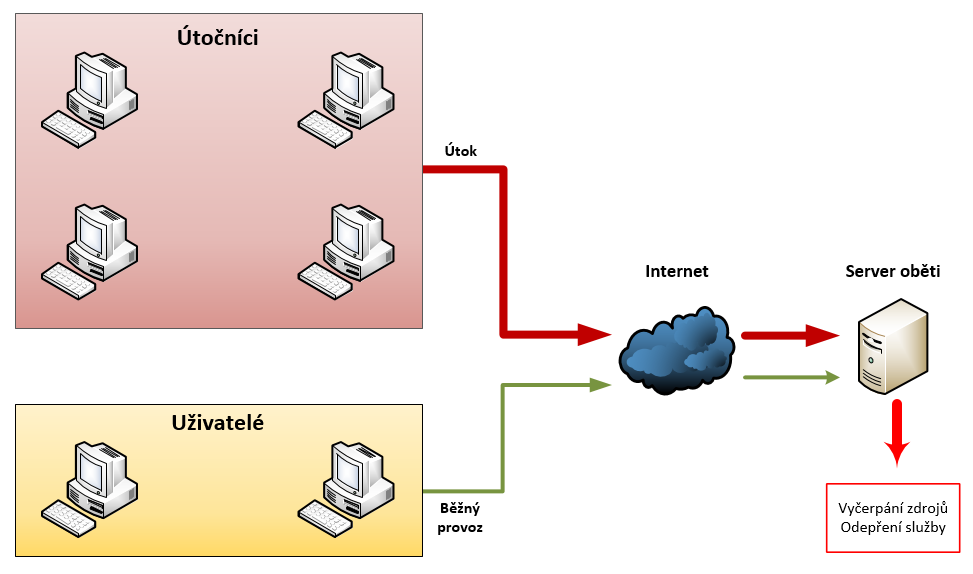
\includegraphics[width=0.99\columnwidth]{obrazky/ddos_schema.png}
			\caption{Schéma DDoS útoku}
		\end{figure}
	\end{column}
\end{columns}											% ukončení prostředí sloupce
\end{frame}

%%%%%%%%%%%%%

\begin{frame}
\frametitle{DoSgen}
\begin{figure}%
	\centering
	\vspace{0.3cm}	              % horizontální mezera
	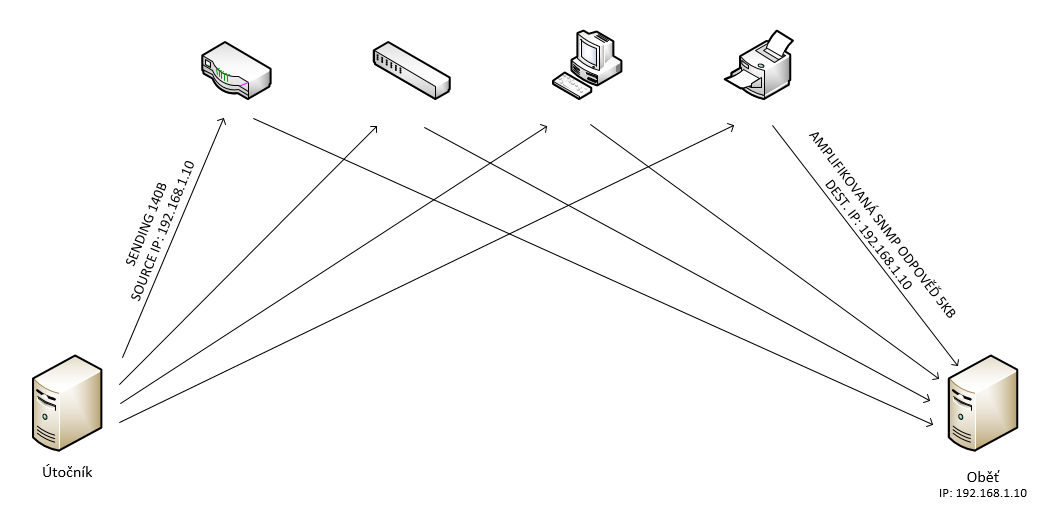
\includegraphics[width=0.9\columnwidth]{obrazky/snmp_flood_schema.png}
	\caption{Schéma amplifikovaného útoku}%
\end{figure}
\end{frame}

%%%%%%%%%%%%%

\begin{frame}
\frametitle{Implementované útoky}

\begin{columns}[T] 								% prostředí sloupce s umístěním nahoře
\begin{column}{0.333333333\textwidth}		% první sloupec
	\begin{itemize}
		\item NTP Flood
		\begin{itemize}
			\item UDP protokol
			\item Reflekce + amplifikace, až 556.9krát
			\item IP spoofing
			\item \texttt{monlist}
			\begin{itemize}
				\item 600 záznamů
			\end{itemize}
		\end{itemize}
	\end{itemize}
\end{column}
%
\begin{column}{0.333333333\textwidth}		% druhý sloupec
	\begin{itemize}
		\item SNMP Flood
		\begin{itemize}
			\item UDP protokol, SNMPv2c
			\item Reflekce + amplifikace, až 6.3krát
			\item Komunikace \\agent - manažer i obráceně
			\item \texttt{community	string} = \textit{public}
			\item \texttt{GetBulkRequest}
		\end{itemize}
	\end{itemize}
\end{column}
%
\begin{column}{0.333333333\textwidth}		% druhý sloupec
	\begin{itemize}
		\item SSDP Flood
		\begin{itemize}
			\item UDP, 1900
			\item Reflekce + amplifikace, až 30.8krát
			\item Komunikace multicast \texttt{239.255.255.250}
			\item UPnP
			\item \texttt{M-SEARCH}, \texttt{NOTIFY}
			\item Odpověď unicast
		\end{itemize}
	\end{itemize}
\end{column}
\end{columns}											% ukončení prostředí sloupce
\end{frame}

%%%%%%%%%%%%%

%\begin{frame}
%	\frametitle{NTP Flood}
%	
%	\begin{columns}[T] 								% prostředí sloupce s umístěním nahoře
%		\begin{column}{0.4\textwidth}		% první sloupec
%			\begin{itemize}
%				\item UDP protokol
%				\item Reflekce + amplifikace, až 556.9krát
%				\begin{itemize}
%					\item IP spoofing
%				\end{itemize}
%				\item \texttt{monlist}
%				\begin{itemize}
%					\item monitorování
%					\item 600 klientů
%				\end{itemize}
%				\item mapování ze strany útočníků
%				\item situace dnes
%				\begin{itemize}
%					\item CVE-2013-5211
%				\end{itemize}
%			\end{itemize}
%		\end{column}
%		%
%		\begin{column}{0.6\textwidth}		% druhý sloupec
%			\begin{figure}%	
%				\centering
%				\vspace{1cm}	              % horizontální mezera
%				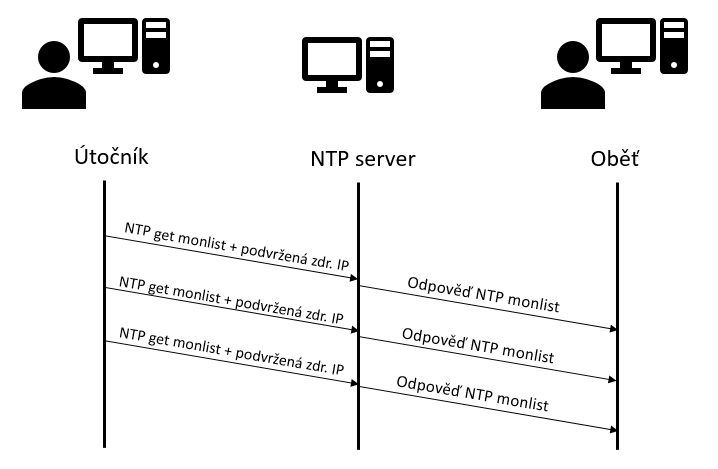
\includegraphics[width=0.8\columnwidth]{obrazky/ntp_flood_schema.png}
%			\end{figure}
%		\end{column}
%	\end{columns}											% ukončení prostředí sloupce
%\end{frame}


%%%%%%%%%%%%%
\begin{frame}
\frametitle{Násobení velikosti odpovědi oproti požadavku}
\vspace{0.1cm}
\begin{table}[ht]
\centering
\caption{Amplifikační útoky založené na UDP}
\label{tab:udp_ampl}
\begin{tabular}{|l|l|}
\hline
\textbf{Protokol}      & \textbf{Faktor zvětšení šířky pásma}    \\ \hline
NTP                    & 556.9                                   \\ \hline
CharGen                & 358.8                                   \\ \hline
DNS                    & do 179                                  \\ \hline
QOTD                   & 140.3                                   \\ \hline
Quake Network Protocol & 63.9                                    \\ \hline
BitTorrent             & 4.0 - 54.3                              \\ \hline
SSDP                   & 30.8                                    \\ \hline
Kad                    & 16.3                                    \\ \hline
SNMPv2                 & 6.3                                     \\ \hline
\end{tabular}
\end{table}
\end{frame}

%%%%%%%%%%%%%

%\begin{frame}
%\frametitle{SNMP Flood}
%
%\begin{columns}[T] 								% prostředí sloupce s umístěním nahoře
%	\begin{column}{0.4\textwidth}		% první sloupec
%		\begin{itemize}
%			\item UDP protokol, SNMPv2c
%			\item Reflekce + amplifikace, až 6.3krát
%			\item Komunikace \\agent - manažer i obráceně
%			\item \texttt{community	string} = \textit{public}
%			\item \texttt{GetBulkRequest}
%			\item OID 1.3.6.1.2.1.1
%		\end{itemize}
%	\end{column}
%	%
%	\begin{column}{0.6\textwidth}		% druhý sloupec
%		\begin{figure}%
%			\centering
%			\vspace{1cm}	              % horizontální mezera
%			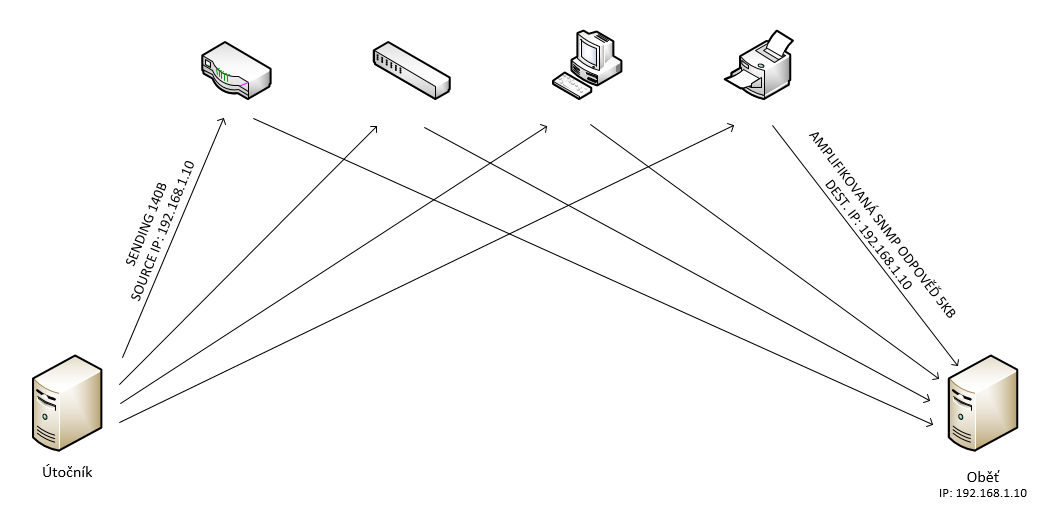
\includegraphics[width=1\columnwidth]{obrazky/snmp_flood_schema.png}
%		\end{figure}
%	\end{column}
%\end{columns}											% ukončení prostředí sloupce
%\end{frame}

%%%%%%%%%%%%%

%\begin{frame} 
%\frametitle{SSDP Flood}
%
%\begin{columns}[T] 								% prostředí sloupce s umístěním nahoře
%	\begin{column}{0.4\textwidth}		% první sloupec
%		%			Obrázek znázorňuje modelfsdfsdfsfasf:\\[2ex]
%		%
%		\begin{itemize}
%			\item UDP, 1900
%			\item Reflekce + amplifikace, až 30.8krát
%			\item Komunikace multicast \texttt{239.255.255.250}
%			\item UPnP
%			\item \texttt{M-SEARCH}, \texttt{NOTIFY}
%			\item HTTP hlavička
%			\item Odpověď unicast
%		\end{itemize}
%	\end{column}
%	%
%	\begin{column}{0.6\textwidth}		% druhý sloupec
%		\begin{figure}%
%			\centering
%			\vspace{1cm}	              % horizontální mezera
%			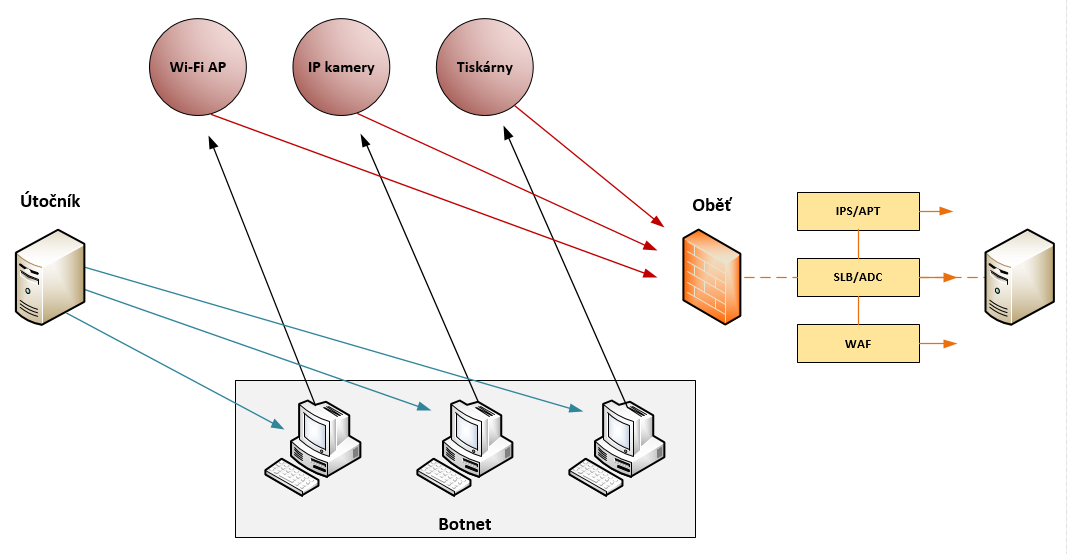
\includegraphics[width=1\columnwidth]{obrazky/ssdp_flood_schema.png}
%		\end{figure}
%	\end{column}
%\end{columns}											% ukončení prostředí sloupce
%\end{frame}
%
%%%%%%%%%%%%%%
%
%\begin{frame}
%\frametitle{SSDP Flood}
%		\begin{figure}%
%			\centering
%			\vspace{0.4cm}	              % horizontální mezera
%			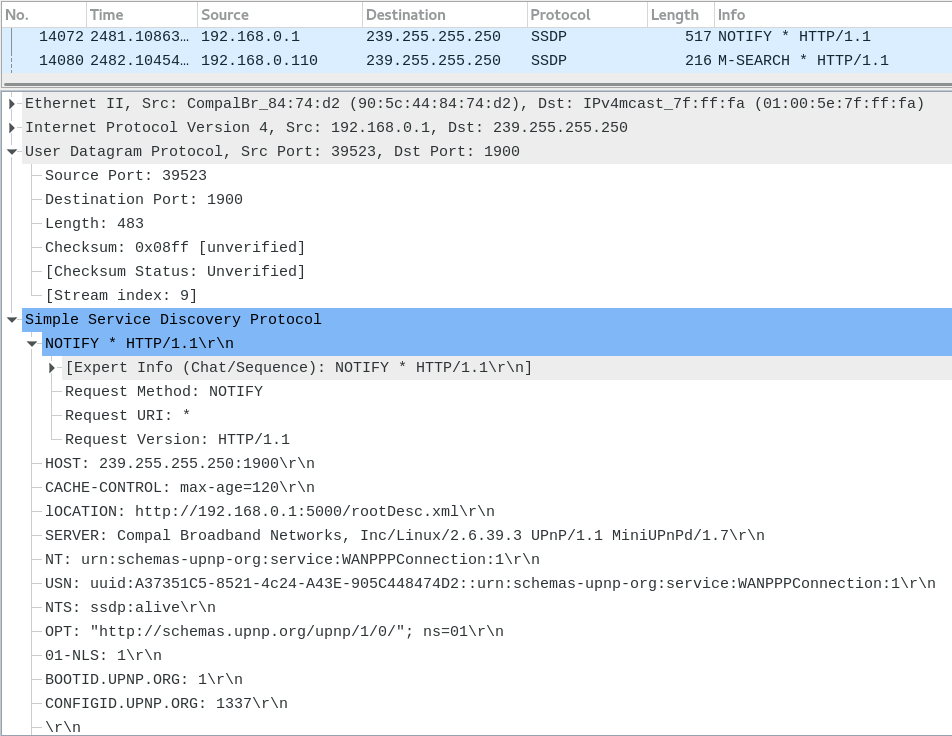
\includegraphics[width=0.659\columnwidth]{obrazky/ssdp_packets_wireshark.png}
%		\end{figure}										% ukončení prostředí sloupce
%\end{frame}

%%%%%%%%%%%%%

\begin{frame}
\frametitle{DoSgen}
\begin{columns}[T] 								% prostředí sloupce s umístěním nahoře
\begin{column}{0.4\textwidth}		% první sloupec
\begin{itemize}
\item Implementace v C, \CC
\item \texttt{trafgen}
\begin{itemize}
	\item \texttt{netsniff-ng}
	\item zero-copy
	\item více jader
\end{itemize}
\item Webové rozhraní
\begin{itemize}
	\item Node.js
	\item HTTPS, 8888
\end{itemize}
\end{itemize}
\end{column}
%
\begin{column}{0.6\textwidth}		% druhý sloupec
\begin{figure}
\centering
\vspace{0.3cm}	              % horizontální mezera
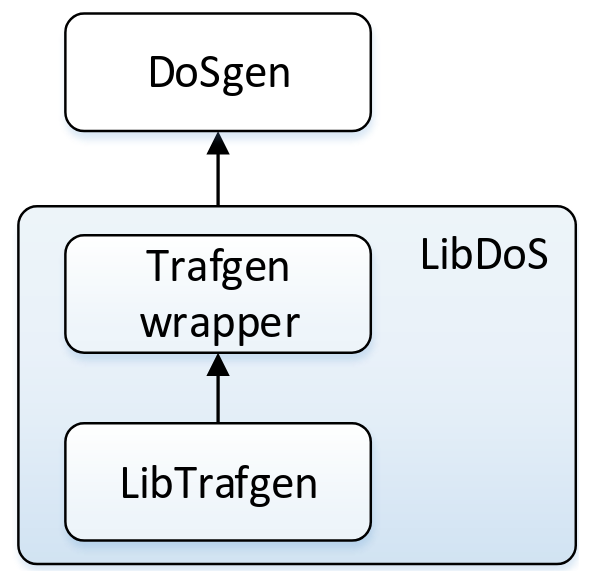
\includegraphics[width=0.6\columnwidth]{obrazky/dosgen_halaska_diagrampng.png}
\caption{Struktura aplikace DoSgen}%
\end{figure}
\end{column}
\end{columns}
\end{frame}

%%%%%%%%%%%%%

\begin{frame}
\frametitle{DoSgen webové rozhraní}
	\begin{itemize}
		\item Aktualizace závislostí (CVE)
		\item Aktualizace inicializačního skriptu (systemd)
		\item Implementace útoků
	\end{itemize}
	\begin{figure}%
		\centering
		\vspace{0.25cm}	              % horizontální mezera
		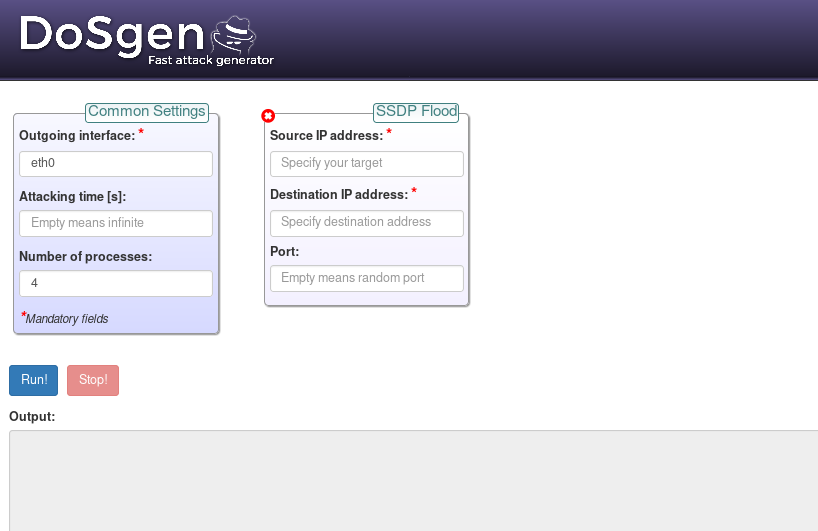
\includegraphics[width=0.5\columnwidth]{obrazky/dosgen-webui.png}
		\caption{Hlavní stránka webového rozhraní aplikace DoSgen}%
	\end{figure}
\end{frame}

%%%%%%%%%%%%%

\begin{frame}
\frametitle{DoSgen nástoroje, dokumentace}
\begin{itemize}
\item Ansible playbooks
\begin{itemize}
\item Prerekvizity útoku
\end{itemize}
\item Kickstart file
\item man stránka
\begin{itemize}
\item Markdown → roff
\end{itemize}
\item Pomocné skripty (fake\_ntp\_hosts.py, \dots)
\item Dokumentace v příloze práce
\end{itemize}
\end{frame}

%%%%%%%%%%%%%

\begin{frame}
\frametitle{Testování}
	\begin{figure}%
	\centering
	%\vspace{0.1cm}	              % horizontální mezera
	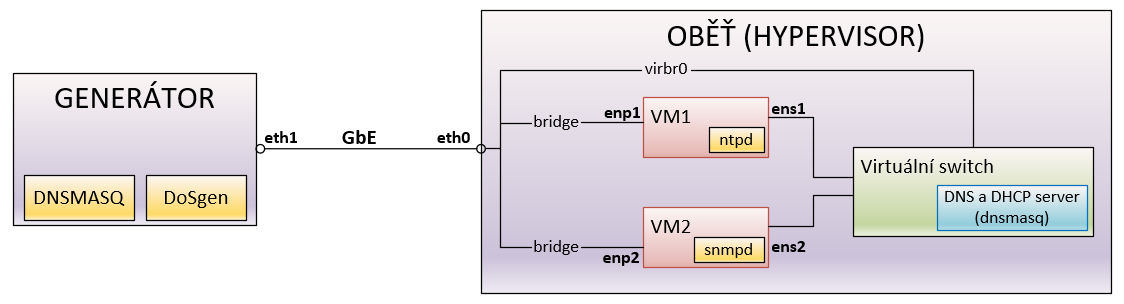
\includegraphics[width=0.659\columnwidth]{obrazky/lab_schema.png}
	\caption{Schéma zapojení testovací sítě.}
	\begin{table}[ht]
		\centering
		\caption{Propustnost mezi jednotlivými rozhraními (uvedeno v Mb/s).}
		\label{tab:troughput-lab-interfaces}
	\begin{tabular}{|l|l|l|l|l|}
		\hline
		Rozhraní & eth1 & eth0  & enp1  & ens1  \\ \hline
		eth1     &      & 941   & 525   & 940   \\ \hline
		eth0     & 941  &       & 19200 & 19200 \\ \hline
		enp1     & 525  & 19200 &       & 19200 \\ \hline
		ens1     & 940  & 19200 & 19200 &       \\ \hline
	\end{tabular}
	\end{table}
	\end{figure}
\end{frame}

%%%%%%%%%%%%%

\begin{frame}
\frametitle{Testování}

\begin{figure}%
	\centering
	\vspace{0.4cm}	              % horizontální mezera
	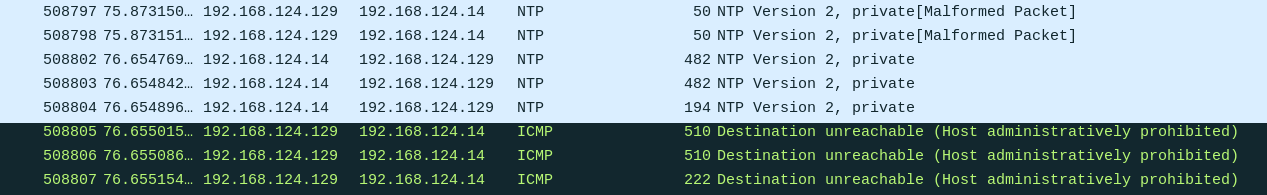
\includegraphics[width=0.99\columnwidth]{obrazky/mon_getlist_1_wireshark_with_icmp_and_reply.png}
	\caption{Průběh NTP útoku zobrazený v aplikaci Wireshark.}
\end{figure}

\begin{figure}%
	\centering
	\vspace{0.4cm}	              % horizontální mezera
	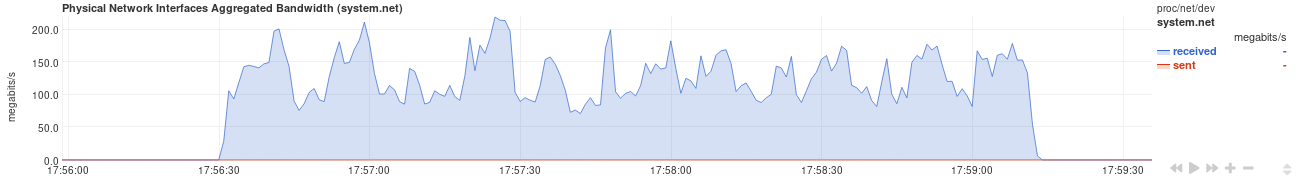
\includegraphics[width=0.99\columnwidth]{obrazky/grafy/graph_ntp_traffic_5ampl.png}
	\caption{Průběh NTP útoku s 5 NTP servery, síťový provoz na straně oběti.}
\end{figure}
\end{frame}

%%%%%%%%%%%%%

\begin{frame}
\frametitle{Testování}
\begin{figure}%
	\centering
	\vspace{0.2cm}	              % horizontální mezera
	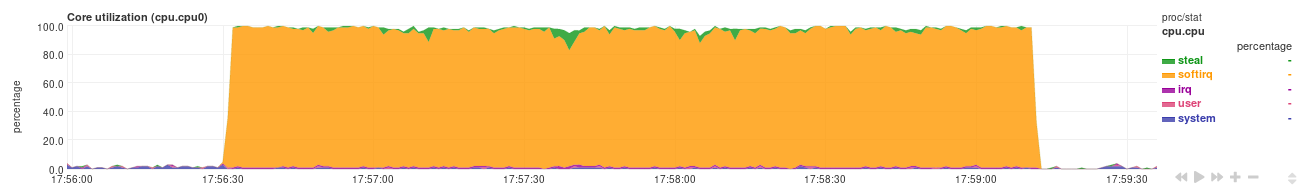
\includegraphics[width=0.99\columnwidth]{obrazky/grafy/graph_ntp_cpu_5ampl.png}
	\caption{Průběh NTP útoku s 5 NTP servery, zatížení CPU na straně oběti.}
\end{figure}

\begin{figure}%
	\centering
	\vspace{0.2cm}	              % horizontální mezera
	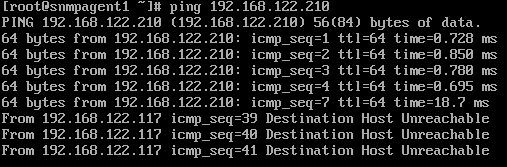
\includegraphics[width=0.6\columnwidth]{obrazky/grafy/ping_ntp_5ampl.png}
	\caption{Test odezvy stanice (oběti), ICMP ping.}
\end{figure}
\end{frame}

%%%%%%%%%%%%%

\begin{frame}
\frametitle{Testování}
\begin{itemize}
	\item Otestovány všechny útoky
	\begin{itemize}
		\item Konfigurace paketu 
	\end{itemize}
	\item Složitější nastavení infrastruktury
	\item Potřeba většího počtu zařízení
	\item Testování na fyzické infrastruktuře vhodnější
	\begin{itemize}
		\item Potíže s virtuálním switchem
		\item Nedošlo k DoS
	\end{itemize}
\end{itemize}

\begin{figure}%
	\centering
	\vspace{0.4cm}	              % horizontální mezera
	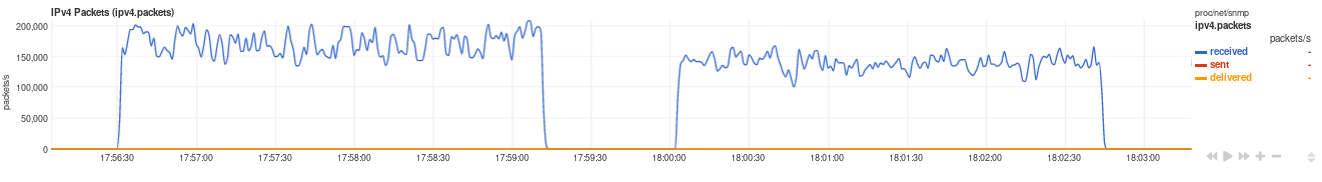
\includegraphics[width=0.92\columnwidth]{obrazky/grafy/graph_ntp_traffic_5ampl_vs6ampl.png}
	\caption{Porovnání průběhu NTP útoku s 5 a 6 NTP servery, síťový provoz - oběť.}
\end{figure}
\end{frame}

%%%%%%%%%%%%%

\begin{frame} 
\frametitle{Závěr}
\begin{itemize}
\item Teoretický popis útoků
\item Popis implementovaných útoků
\begin{itemize}
\item Mitigace
\end{itemize}
\item Rozšíření nástroje DoSgen
\item Rozšíření webového rozhraní
\item Dokumentace, pomocné nástroje
\item Nastavení, konfigurace testovacího prostředí
\item Implementováno a otestováno

\item Budoucí rozšíření možné, složitější
\end{itemize}
\end{frame}

%%%%%%%%%%%%%

% podekovani
\begin{frame}[c] 
% bez nadpisu snimku
\frametitle{\mbox{ }}
\begin{center}
{\Huge Děkuji za pozornost!}
\end{center}
\end{frame}

% otázky oponenta
\frame{
\frametitle{Otázky oponenta}
\emph{Měl na dosahované výsledky měření vliv spuštěný program Wireshark?}\\[1ex]
%
Při získávání výsledků program Wireshark spuštěn nebyl právě proto, abych eliminoval veškeré možné aspekty, které by měly negativní vliv na výsledky měření.
Wireshark, tedy \texttt{libpcap}, při spuštění útoku však vykazoval značné zpoždění při zobrazování zachycených paketů. Je tedy možné, že některé ze statisíců paketů \texttt{libpcap} nezachytil.
\\[3ex]

\emph{Na jakém rozhraní byly pakety zachytávány při jednotlivých testech?}\\[1ex]
%
Při ladění konfigurace paketu nástroje DoSgen byly pakety zachytávány na stanici, jež dané pakety přijímala. Důvodem byla nemožnost zachytávat pakety na rozhraní generátoru, jelikož trafgen pracuje pouze v prostoru jádra OS, kdežto Wireshark v uživatelském prostoru.
Na této stanici bylo možno zachytit jak paket odeslaný generátorem, tak případnou odpověď oběti.
}

\end{document}
